% Options for packages loaded elsewhere
\PassOptionsToPackage{unicode}{hyperref}
\PassOptionsToPackage{hyphens}{url}
%
\documentclass[
  ignorenonframetext,
]{beamer}
\usepackage{pgfpages}
\setbeamertemplate{caption}[numbered]
\setbeamertemplate{caption label separator}{: }
\setbeamercolor{caption name}{fg=normal text.fg}
\beamertemplatenavigationsymbolsempty
% Prevent slide breaks in the middle of a paragraph
\widowpenalties 1 10000
\raggedbottom
\setbeamertemplate{part page}{
  \centering
  \begin{beamercolorbox}[sep=16pt,center]{part title}
    \usebeamerfont{part title}\insertpart\par
  \end{beamercolorbox}
}
\setbeamertemplate{section page}{
  \centering
  \begin{beamercolorbox}[sep=12pt,center]{part title}
    \usebeamerfont{section title}\insertsection\par
  \end{beamercolorbox}
}
\setbeamertemplate{subsection page}{
  \centering
  \begin{beamercolorbox}[sep=8pt,center]{part title}
    \usebeamerfont{subsection title}\insertsubsection\par
  \end{beamercolorbox}
}
\AtBeginPart{
  \frame{\partpage}
}
\AtBeginSection{
  \ifbibliography
  \else
    \frame{\sectionpage}
  \fi
}
\AtBeginSubsection{
  \frame{\subsectionpage}
}
\usepackage{lmodern}
\usepackage{amssymb,amsmath}
\usepackage{ifxetex,ifluatex}
\ifnum 0\ifxetex 1\fi\ifluatex 1\fi=0 % if pdftex
  \usepackage[T1]{fontenc}
  \usepackage[utf8]{inputenc}
  \usepackage{textcomp} % provide euro and other symbols
\else % if luatex or xetex
  \usepackage{unicode-math}
  \defaultfontfeatures{Scale=MatchLowercase}
  \defaultfontfeatures[\rmfamily]{Ligatures=TeX,Scale=1}
\fi
% Use upquote if available, for straight quotes in verbatim environments
\IfFileExists{upquote.sty}{\usepackage{upquote}}{}
\IfFileExists{microtype.sty}{% use microtype if available
  \usepackage[]{microtype}
  \UseMicrotypeSet[protrusion]{basicmath} % disable protrusion for tt fonts
}{}
\makeatletter
\@ifundefined{KOMAClassName}{% if non-KOMA class
  \IfFileExists{parskip.sty}{%
    \usepackage{parskip}
  }{% else
    \setlength{\parindent}{0pt}
    \setlength{\parskip}{6pt plus 2pt minus 1pt}}
}{% if KOMA class
  \KOMAoptions{parskip=half}}
\makeatother
\usepackage{xcolor}
\IfFileExists{xurl.sty}{\usepackage{xurl}}{} % add URL line breaks if available
\IfFileExists{bookmark.sty}{\usepackage{bookmark}}{\usepackage{hyperref}}
\hypersetup{
  pdftitle={Giving Price, Governement Expenditure, and Political Trust},
  pdfauthor={Hiroki Kato\^{}1; Tsuyoshi Goto\^{}2; Yong-Rok Kim\^{}3},
  hidelinks,
  pdfcreator={LaTeX via pandoc}}
\urlstyle{same} % disable monospaced font for URLs
\newif\ifbibliography
\usepackage{graphicx}
\makeatletter
\def\maxwidth{\ifdim\Gin@nat@width>\linewidth\linewidth\else\Gin@nat@width\fi}
\def\maxheight{\ifdim\Gin@nat@height>\textheight\textheight\else\Gin@nat@height\fi}
\makeatother
% Scale images if necessary, so that they will not overflow the page
% margins by default, and it is still possible to overwrite the defaults
% using explicit options in \includegraphics[width, height, ...]{}
\setkeys{Gin}{width=\maxwidth,height=\maxheight,keepaspectratio}
% Set default figure placement to htbp
\makeatletter
\def\fps@figure{htbp}
\makeatother
\setlength{\emergencystretch}{3em} % prevent overfull lines
\providecommand{\tightlist}{%
  \setlength{\itemsep}{0pt}\setlength{\parskip}{0pt}}
\setcounter{secnumdepth}{-\maxdimen} % remove section numbering
\setbeamertemplate{navigation symbols}{}
\setbeamertemplate{footline}[page number]

\usepackage{bookmark}
\usepackage{booktabs}

\usepackage{xltxtra} 
\usepackage{zxjatype} 
\usepackage[ipa]{zxjafont} 
\ifluatex
  \usepackage{selnolig}  % disable illegal ligatures
\fi

\title{Giving Price, Governement Expenditure, and Political Trust}
\author{Hiroki Kato\(^1\) \and Tsuyoshi Goto\(^2\) \and Yong-Rok
Kim\(^3\)}
\date{2021/01/10}
\institute{\(^1\)Osaka University \and \(^2\)Chiba
University \and \(^3\)Kobe University}

\begin{document}
\frame{\titlepage}

\hypertarget{introduction}{%
\section{Introduction}\label{introduction}}

\begin{frame}{Charitable Giving and Governement Policy}
\protect\hypertarget{charitable-giving-and-governement-policy}{}
There are huge literatures to investigate relationship bewteen chariable
giving and governement policies

\begin{enumerate}
\tightlist
\item
  price elasticity of charitable giving using the tax benefit
\item
  the crowd-out effect of government expenditure
\end{enumerate}

Even though tax benefits directly affect government expenditure, there
is no literature to try to connect the tax benefit with governement
expenditure as far as we know.

We investigate the price effect and the crowd-out effect simultaneously,
and connect two effects through political trust.
\end{frame}

\begin{frame}{Why Political Trust?}
\protect\hypertarget{why-political-trust}{}
We conjecture that the political trust is key driver to determine the
price effect and the crowd-out effect

\begin{itemize}
\tightlist
\item
  Price effect: If people untrust politicians, then they may also
  suspect the system of tax banefit. If people trust politicians
  sufficiently, then they may try to send money to government. Thus,
  they do not use the tax benefit which decreases governement's revenue.
\item
  Crowd-out effect: If people untrust politicians, then they may expect
  that governement does not invest the public goods. This is related
  with the strategic uncertainty.
\end{itemize}
\end{frame}

\begin{frame}{Background of South Korea Tax Reform}
\protect\hypertarget{background-of-south-korea-tax-reform}{}
To investigate the price effect, we use the 2014 tax reform in the South
Korea.

\begin{itemize}
\tightlist
\item
  Before 2014, tax deduction was adopted to subsidize charitable
  donation behavior.
\item
  After 2014, tax credit have been adopted.
\end{itemize}

The main difference is that tax credits reduce taxes directly, while tax
deductions indirectly lower the tax burden by decreasing the taxpayer's
marginal tax rate, which increases with gross income
\end{frame}

\hypertarget{data}{%
\section{Data}\label{data}}

\begin{frame}{Data Source}
\protect\hypertarget{data-source}{}
To construct dataset, we use two surveys:

\begin{enumerate}
\tightlist
\item
  National Survey of Tax and Benefit (NaSTaB)
\item
  Data on local government finance from Ministry of the Interior and
  Safety (MIS data)
\end{enumerate}
\end{frame}

\begin{frame}{National Survey of Tax and Benefit (NaSTaB)}
\protect\hypertarget{national-survey-of-tax-and-benefit-nastab}{}
\begin{itemize}
\tightlist
\item
  The Korea Institute of Taxation and Finance implements the financial
  panel survey to study the tax burden of households and the benefits
  that households receive from goverment.
\item
  The subjects of this survey are general household and household
  members living in 15 cities and provinces nationwide.
\item
  This survey is based on a face-to-face interview. If it is difficult
  for investigators to meet subjects, another family member answers on
  behalf of him.
\item
  Survey items: Annual taxable income (last year), charitable donations
  (last year), trust for politicians (5-Likert scale), and other
  covariates (age, education, gender etc.).
\item
  Survey period: 2008 \textasciitilde{} 2019

  \begin{itemize}
  \tightlist
  \item
    We use survey data after 2013 to focus on tax policy change in 2014.
  \end{itemize}
\end{itemize}
\end{frame}

\begin{frame}{MIS data}
\protect\hypertarget{mis-data}{}
\begin{itemize}
\tightlist
\item
  MIS of South Korean collects data on local governement finance.
\item
  From this data, we obtain infomation about tax revenue and expenditure
  for social welfare.
\item
  Using the population data, we calculate the local governement
  expenditure per capita and use this variable as main explanatory
  variable.
\item
  Since the NaSTab includes residence area of respondents, it merges
  with the data on local governement finance.
\end{itemize}
\end{frame}

\begin{frame}{Variable of Giving Price}
\protect\hypertarget{variable-of-giving-price}{}
In the South Korea, the tax policy about charitable giving drastically
changed in 2014. Before 2014, the \textbf{tax deduction} adpoted. After
2014, the \textbf{tax credit} adopted. Under two systems, the giving
price is

\begin{itemize}
\tightlist
\item
  tax deduction: \(\text{Price} = 1 - \tau\)
\item
  tax credit: \(\text{Price} = 1 - r\)
\end{itemize}

\(\tau\) is the marginal income tax rate calculated by annual taxable
income reported in the NaSTaB, and \(r\) is the tax credit rate
determined exogeneity. In the South Korea, \(r = 0.15\).
\end{frame}

\hypertarget{results}{%
\section{Results}\label{results}}

\begin{frame}{Trust Index}
\protect\hypertarget{trust-index}{}
The trust for politicans is time-varying variable because it depends on
governments' policies. We make time-invarying trust index using the
fixed effect model.

\[
    \text{Trust}_{ijt} = \text{Trustid}_i + c_j \cdot \lambda_t + \lambda_t + \epsilon_{ijt}.
\]

\begin{itemize}
\tightlist
\item
  \(\text{Trust}_{ijt}\): trust for politicians (5-Likert scale)
\item
  \(\text{Trustid}_i\): individual fixed effect (\textbf{Trust index})
\item
  \(c_j \cdot \lambda_t\) captures local governments' policies effect
\item
  \(\lambda_t\) captures the central government policies effect
\end{itemize}

We rescale the trust index to an interval \([0,1]\).
\end{frame}

\begin{frame}{Histrogram of Trust Index}
\protect\hypertarget{histrogram-of-trust-index}{}
\begin{figure}
\centering
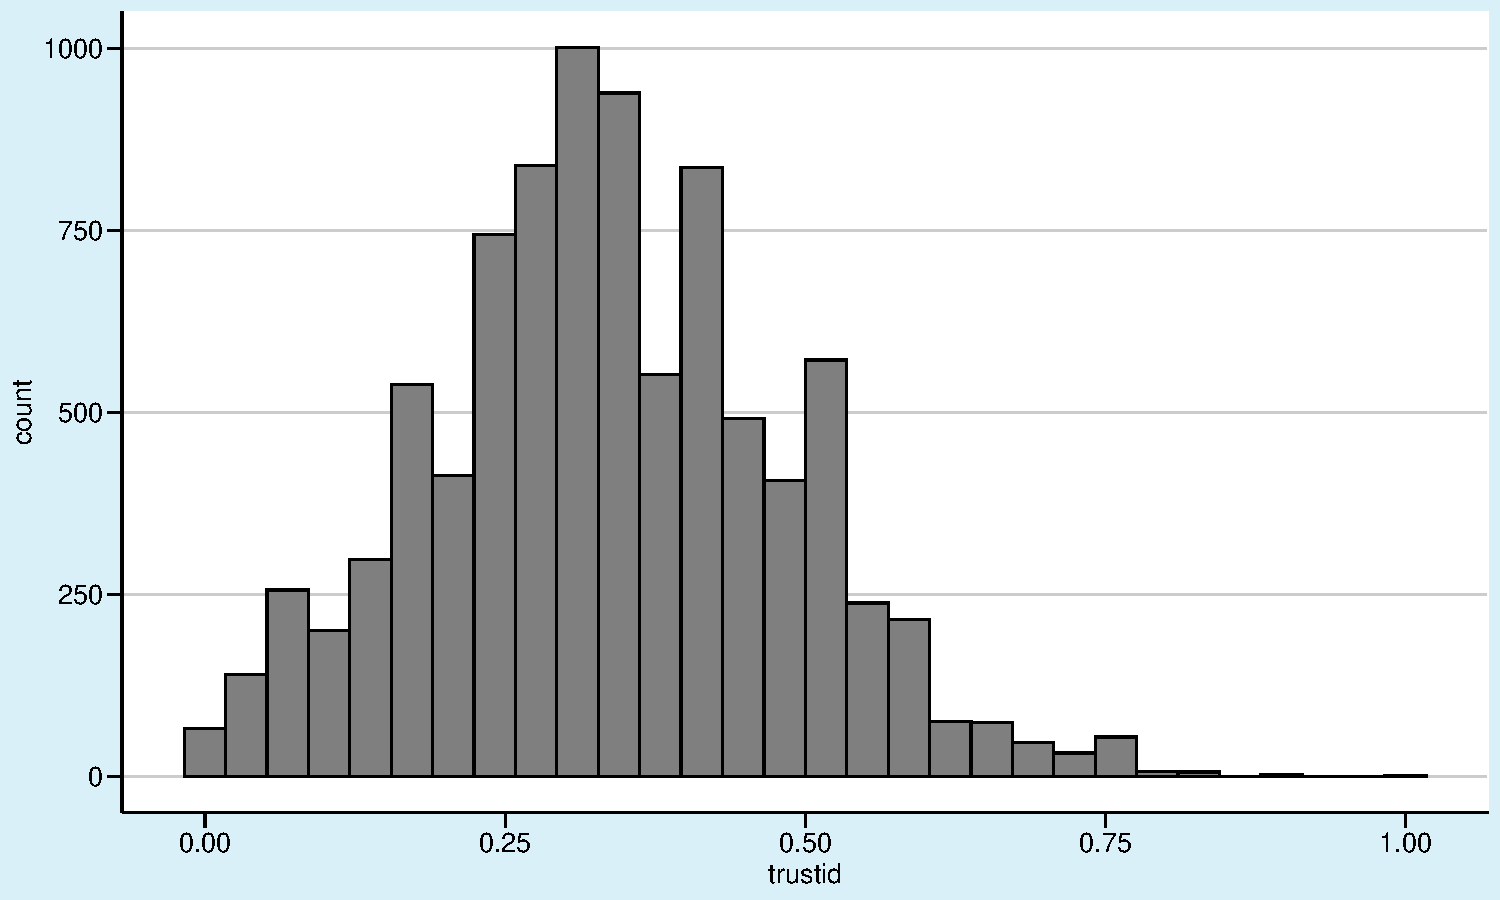
\includegraphics{C:/Users/katoo/Desktop/NASTAB/report/slides_files/figure-beamer/TrustIndex-1.pdf}
\caption{Histogram of Trust Index}
\end{figure}
\end{frame}

\begin{frame}{Regression of Trust Index}
\protect\hypertarget{regression-of-trust-index}{}
\begin{table}

\caption{\label{tab:kableTabTrustReg}Regression of Trust Index (Year = 2018)}
\centering
\begin{tabular}[t]{lcc}
\toprule
Variables & Coefficients & S.E.\\
\midrule
gender & 0.007** & (0.003)\\
age & -0.003*** & (0.001)\\
I((age/100)\textasciicircum{}2) & 0.311*** & (0.055)\\
factor(educ)2 & 0.004 & (0.005)\\
factor(educ)3 & 0.003 & (0.006)\\
factor(political\_pref)2 & 0.027** & (0.013)\\
factor(political\_pref)3 & 0.033*** & (0.012)\\
factor(political\_pref)4 & 0.021* & (0.013)\\
factor(political\_pref)5 & -0.065*** & (0.014)\\
Obs & 7697 & \\
Adjusted R-sq & 0.0316 & \\
\bottomrule
\end{tabular}
\end{table}
\end{frame}

\begin{frame}{Baseline Regressions}
\protect\hypertarget{baseline-regressions}{}
Our baseline regression equation is

\begin{align*}
    \log(\text{Giving}_{ijt}) = 
    &\alpha_i + \beta_1 \log(\text{Price}_{ijt}) + \beta_2 \log(\text{Expend}_{jt}) \\
    &+ \delta X_{ijt} + \lambda_t + \epsilon_{ijt}.
\end{align*}

\begin{itemize}
\tightlist
\item
  \(\log(\text{Giving}_{ijt})\) is logarithm of individual \(i\)'s
  charitable giving in year \(t\).
\item
  \(\log(\text{Price}_{ijt})\) is logarithm of individual \(i\)'s giving
  price in year \(t\).
\item
  \(\log(\text{Expend}_{jt})\) is local government \(j\)'s expenditure
  for social welfare in year \(t\).
\item
  \(\beta_1\) represents the price elasticity of giving.
\item
  \(\beta_2\) represents the local government expenditure elasticity of
  giving.
\item
  \(\alpha_i\) and \(\lambda_t\) are individual and time fixed effect,
  respectively.
\end{itemize}
\end{frame}

\begin{frame}{Result of Baseline Regressions}
\protect\hypertarget{result-of-baseline-regressions}{}
\begin{table}

\caption{\label{tab:kableTabBaseReg}Baseline Regressions}
\centering
\begin{tabular}[t]{lccc}
\toprule
 & (1) & (2) & (3)\\
\midrule
ln(giving price) & -1.071*** & -1.059*** & -1.062***\\
 & (0.201) & (0.226) & (0.226)\\
Year X Educ & N & Y & Y\\
Year X Gender & N & Y & Y\\
Living Dummy & N & N & Y\\
Obs & 54213 & 54211 & 54211\\
\bottomrule
\end{tabular}
\end{table}
\end{frame}

\begin{frame}{Interpretations of Baseline Regression}
\protect\hypertarget{interpretations-of-baseline-regression}{}
\begin{itemize}
\tightlist
\item
  We found the \textbf{price effect} of giving (1\% price increase leads
  to about 1.1\% giving decrease)
\item
  We found the \textbf{crowd-in effect} of local government expenditure
  (1\% expenditure increase leads to 0.8\% increase giving)

  \begin{itemize}
  \tightlist
  \item
    This effect is heterogenous by the level of government expenditure.
    As local government expenditure increases, the crowd-in effect
    vanish, and the crowd-out effect emerges.
  \end{itemize}
\end{itemize}
\end{frame}

\begin{frame}{Subgroup Regressions}
\protect\hypertarget{subgroup-regressions}{}
We estimate the baseline regression equation, using sample grouped by
the trust index.

\begin{itemize}
\tightlist
\item
  Lowest: 0 \textasciitilde{} 20\% quantile of trust index
\item
  Lower: 20 \textasciitilde{} 40\% quantile of trust index
\item
  Neutral: 40 \textasciitilde{} 60\% quantile of trust index
\item
  Higher: 60 \textasciitilde{} 80\% quantile of trust index
\item
  Highest: 80 \textasciitilde{} 100\% quantile of trust index
\end{itemize}

We include the logarithm of income, age, interactions b/w year and
education, interactions b/w year and gender, and living are dummy into
covariates.
\end{frame}

\begin{frame}{Results of Subgroup Regressions}
\protect\hypertarget{results-of-subgroup-regressions}{}
\begin{table}

\caption{\label{tab:kableTabTrustGroupReg}Subgroup Regressions}
\centering
\fontsize{9}{11}\selectfont
\begin{tabular}[t]{lccccc}
\toprule
 & Lowest & Lower & Neutral & Higher & Highest\\
\midrule
ln(giving price) & -0.675 & -0.460 & -1.582*** & -1.284** & -1.202**\\
 & (0.556) & (0.458) & (0.481) & (0.530) & (0.503)\\
Obs & 10239 & 10358 & 10367 & 10368 & 12879\\
\bottomrule
\end{tabular}
\end{table}
\end{frame}

\begin{frame}{Interpretations of Subgroup Regressions}
\protect\hypertarget{interpretations-of-subgroup-regressions}{}
\begin{itemize}
\tightlist
\item
  We could \textbf{NOT} find the crowd-in (crowd-out) effect for
  respondents whose trust is very low and very high.

  \begin{itemize}
  \tightlist
  \item
    We found the crowd-in effect for middle group.
  \item
    If the trust for politicians is low, respondents have a willingness
    to provide public goods without governement help.
  \item
    If the trust for politicians is very high, respondents take a
    strategy of free-rides.
  \end{itemize}
\item
  We cound \textbf{NOT} find the price effect for respondents whose
  trust is very low.

  \begin{itemize}
  \tightlist
  \item
    If the trust is very low, respondents do not want to use a tax
    benefit policies.
  \end{itemize}
\end{itemize}
\end{frame}

\begin{frame}{Heterogenity By Political Trust}
\protect\hypertarget{heterogenity-by-political-trust}{}
To capture heterogeneity precisely, we estimate the following regression
equations:

\begin{align*}
    \log(\text{Giving}_{ijt}) = 
    &\alpha_i + \beta_0 \text{Trust}_{ij} \\
    &+ \beta_1 \log(\text{Price}_{ijt}) + \beta_2 \log(\text{Price}_{ijt})\cdot\text{Trust}_{ij} \\
    &+ \beta_3 \log(\text{Expend}_{jt}) + \beta_4 \log(\text{Expend}_{ijt})\cdot\text{Trust}_{ij}\\
    &+ \delta X_{ijt} + \lambda_t + \epsilon_{ijt}.
\end{align*}

\begin{itemize}
\tightlist
\item
  Price elasticity is obtained by
  \(\beta_1 + \beta_2\cdot\text{Trust}_{ij}\).
\item
  Governement expenditure elasticity is obtained by
  \(\beta_3 + \beta_4\cdot\text{Trust}_{ij}\).
\end{itemize}
\end{frame}

\begin{frame}{Result of Heterogeneity By Political Trust (1)}
\protect\hypertarget{result-of-heterogeneity-by-political-trust-1}{}
\begin{table}

\caption{\label{tab:kableTabTrustHeteroReg}Heterogeneity of Political Trust}
\centering
\begin{tabular}[t]{lcc}
\toprule
Variables & Coefficients & S.E.\\
\midrule
ln(giving price) & -0.251 & (0.453)\\
\hspace{1em}X Trust index & -2.551** & (1.167)\\
Obs & 51306 & \\
\bottomrule
\end{tabular}
\end{table}
\end{frame}

\begin{frame}{Result of Heterogeneity of Political Trust (2)}
\protect\hypertarget{result-of-heterogeneity-of-political-trust-2}{}
\begin{table}

\caption{\label{tab:kableTabTrustHetero2Reg}Heterogeneity of Political Trust (include squared term)}
\centering
\begin{tabular}[t]{lcc}
\toprule
Variables & Coefficients & S.E.\\
\midrule
ln(giving price) & 0.840 & (0.752)\\
\hspace{1em}X Trust index & -10.002** & (3.985)\\
\hspace{1em}X Squared trust index & 10.687** & (5.172)\\
Obs & 51306 & \\
\bottomrule
\end{tabular}
\end{table}
\end{frame}

\begin{frame}{Graphical Representation of Heterogeneity Effect}
\protect\hypertarget{graphical-representation-of-heterogeneity-effect}{}
\begin{figure}
\centering
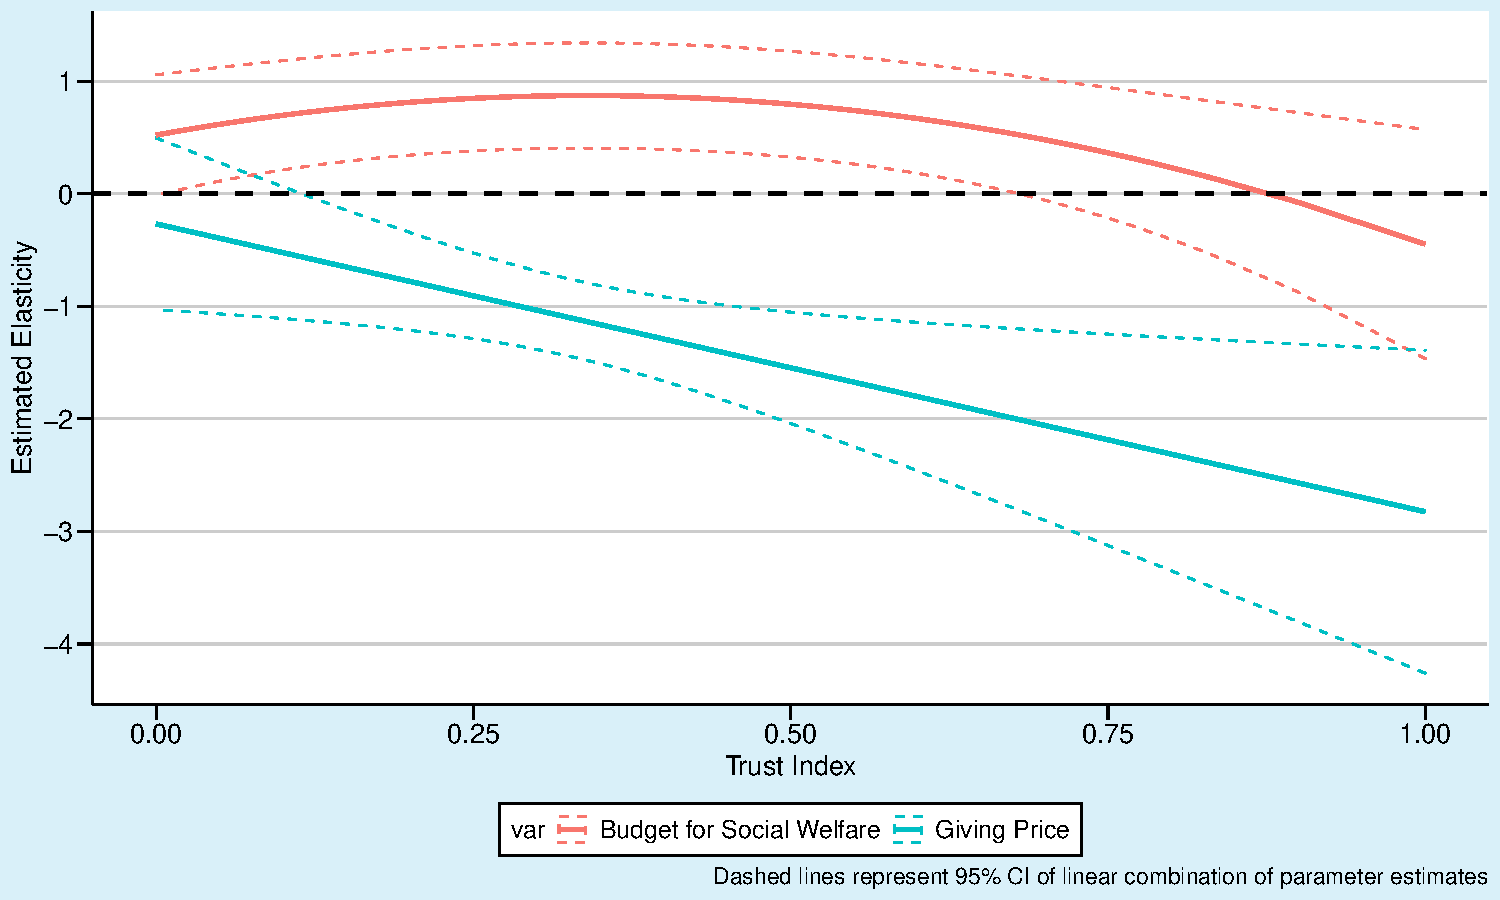
\includegraphics{C:/Users/katoo/Desktop/NASTAB/report/slides_files/figure-beamer/PlotPredictedElast-1.pdf}
\caption{Relationship between Trust Index and Predicted Elasticity}
\end{figure}
\end{frame}

\hypertarget{conclusions}{%
\section{Conclusions}\label{conclusions}}

\begin{frame}{Conclusions}
\protect\hypertarget{conclusions-1}{}
Our primitive result can be summarized as follows:

\begin{itemize}
\tightlist
\item
  Low trust: Since people untrust governement's behavior, they act
  regardless of governement's policies (expenditure and tax benefit)
\item
  Middle trust: Since people have strategic uncertainty, they take a
  strategy of conditional cooperation. That is, they increase donations
  and use tax benefit to boost their giving if a local governement
  increases expenditures.
\item
  High trust (very weak evidence): Since people believe that governement
  contributes to social welfare, they send money to governement (not
  charities). Thus, they hestitate to use a tax benefit compared with
  those whose trust is middle level.
\end{itemize}
\end{frame}

\begin{frame}{Avenue of Our Research}
\protect\hypertarget{avenue-of-our-research}{}
Our primitive results have several serious problem.

\begin{enumerate}
\tightlist
\item
  Endogeneity of giving price. The giving price includes decision-making
  of use of tax benefit.
\item
  Does charitable giving contributes to local social welfare? To examine
  the crowd-out effect of local government expenditure, we need to
  assume that peole send money to charities which work for local social
  welfare.
\item
  Does people believe that a tax benefit decreases the \textbf{local}
  governement's revenue? To interpret our primitive results, we assume
  that people believe that a tax benefit decreases the budget of local
  governement.
\end{enumerate}

In future, we need to solve these problems.
\end{frame}

\end{document}
